\section{Blackboard}


Das Blackboard Pattern ist nützlich für Probleme bei denen keine deterministische Lösungsstrategien bekannt sind. Dabei sammeln mehrere speziallisierte Subsyteme ihr Wissen um eine mögliche Teil- oder Annäherungslösungs zu konstruieren.

\subsection*{Beispiel}


Software für Spracherkennung. Um aus aufgezeichneten Schallwellen Laute, Wörter oder gar sinnvolle Sätze zu transformieren benötigt es verschiedene Prozeduren mit hohen fachlichen Fähigkeiten. Diese Prozeduren arbeiten in verschiedenen Domänen. Wir nehmen an, dass dabei kein passender Algorithmus existiert, welche alle notwendigen Prozeduren zur Spracherkennung kombiniert.

\subsection*{Context}


Eine unreife (unerforschte) Domäne in welchem keine gute Annäherung an eine Lösung bekannt oder machbar ist.

\subsection*{Problem}


Das Blackboard Pattern packt Probleme an, für die keine machbare, deterministische Lösung existiert, wie zum Beispiel die Transformation von rohen Daten in höhere Datenstrukturen, wie Diagramme, Tabellen oder Sätze in einer natürlichen Sprache. Solche Probleme tretten unter anderem in Domänen der Optik, der Bilderkennung, der Spracherkennung oder der Überwachung ein. Diese sind charakterisiert durch ein Problem welches, wenn es in Teilprobleme zerlegt wird, mehrere Fachkompetenzen umfasst. Die Lösungen zu den Teilproblemen benötigen verschiedene Repräsentationen und Modelle. In vielen Fällen existiert keine vorgegebene Strategie wie die Lösungen der Teilprobleme kombiniert werden können.

In einigen Problemdomänen kann es nötig sein mit unsicheren oder angenäherten Lösungen zu arbeiten. Jeder Transformationsschritt könnte auch mehere alternative Lösungen generieren. In diesem Fall ist es oft ausreichend eine optimale Lösung für die meisten Fälle, eine suboptimale Lösung oder garkeine Lösung für den Rest zu finden. Die Einschränkungen eines Blackboard-Systems müssen daher sorgfältig dokumentiert werden und falls wichtige Entscheidungen von dessen Resultaten abhängen, müssen die Resultate sorgfältig überprüft werden.

\subsection*{Forces}


\begin{itemize}
	\item Ein kompletes Durchsuchen des Lösungsraums ist nicht machbar in angemessener Zeit.
	\begin{itemize}
		\item z.B. ein Satz mit 10 Wörtern aus einem Wörterbuch mit 1000 Wörter ergibt 1000\^10 Permutationen
	\end{itemize}
	\item Da die Domäne noch unerforscht (immature) ist, ist es nötig mit verschidenen Algorithmen für die selbe Unteraufgabe zu experimentieren. Dazu müssen die individuellen Module einfach austauschbar sein.
	\item Es gibt verschiedene Algorithmen welche Teilprobleme lösen.
	\begin{itemize}
		\item z.B. die Erkennung von Lauten in gesprochener Sprache ist unabhängig von der semantische Analyse von Sätzen
	\end{itemize}
	\item Eingaben, Zwischen- und Endresultate haben verschidene Repräsentationen. Die Algorithmen sind gemäss den verschiedenen Modellen implementiert.
	\item Ein Algorithmus verarbeitet normalerweise die Resultate eines anderen.
	\item Unsichere Daten und angenäherte Lösungen sind beteiligt. Daten können unerwünschtes "Rauschen" enthalten und das Interpretieren von Signalen ist auch fehleranfällig.
	\item Das Anwenden von unabhängigen Algorithmen kann parallelisiert werden. Nach Möglichkeit sind strikte sequenzielle Lösungen zu vermeiden.
\end{itemize}

Systeme mit Künstlicher Intelligenz (Artifical Intelligence) können ebenfalls eingesetzt werden für solche komplexen nicht-deterministischen Probleme. Dieser Ansatz ist für das Spracherkennungsproblem allerdings weniger geeignet, da Wissenfragmente zu einer bestimmen Zeit angewendet werden müssen, und nicht in einer bestimmten Reihenfolge.

\subsection*{Solution}


Die Idee hinter der Blackboard Architektur ist, dass eine Gruppe von unabhängigen Programmen kooperativ an einer gemeinsamen Datenstruktur arbeitet. Jedes Programm ist spezialisiert einen bestimmten Teil der übergeordneten Aufgabe zu Lösen und alle Programme arbeiten zusammen an der Lösung. Sie rufen sich dabei nicht gegenseitig auf, noch gibt es eine vorgegebene Sequenz für ihre Aktivierung. Eine zentrale Kontrollkomponente beurteilt dabei den aktuellen Zustand der Verarbeitung und koordiniert die spezialisierten Programme. Dieses Art der datengesteuerte (data-directed) Verwaltung wird als \textit{opportunistic problem solving} bezeichnet.

Die Menge aller möglichen Lösungen wird als Solution Space(Lösungsraum) bezeichnet und ist in Abstraktionsstufen organisiert. Die niedrigste Abstraktionsstufe enthält dabei die interne Repräsentation der Eingabe (input). Potentielle Lösungen des Gesamtsystems sind auf der höchsten Stufe.

Der Name Blackboard kommt dabei von der Situation bei der menschliche Experten vor einem Blackboard sitzen und zusammen ein Problem lösen. Jeder Experte bewertet dabei den aktuellen Zustand der Lösung und geht jederzeit möglicherweise ans Blackboard um Informationen hinzuzufügen, ändern oder zu entfernen. Menschen entscheiden normalerweise selbstständig wer als nächstes ans Blackboard geht. Im beschriebenen Pattern entscheidet eine \textit{moderator} Komponente die Reihenfolge in welcher die Programme ausgeführt werden, wenn mehr als ein Programm zurzeit einen Beitrag leisten kann.


\subsection*{Structure}


Unterteile dein System in eine Komponente namens "Blackboard", eine Kollektion von Knowledge Sources (Wissensquellen) und eine Control Component (Kontroll-Komponente).

Das Blackboard ist der zentralle Datenspeicher. Wir nennen die Menge aller Daten welche auf den Blackboard erscheinen kann das \textit{Vocabulary}. Das Blackboard besitzt eine Schnittstelle mit welcher alle Knowledge Sources auf dem Blackboard lesen und schreiben können.

Alle Element aus dem Solution Space (Lösungsraum) können auf dem Blackboard erscheinen. Lösungen welche während dem Problemlösungsprozess erzeugt und auf das Blackboard geschrieben werden heissen Hypothesis (Hypothese) oder Blackboard Entry. Hypothesen welche später verworfen werden, werden vom Blackboard entfernt.

Hypothesen haben normalerweise mehrere Attribute, zum Beispiel die Abstraktionsstufe (abstraction level). Weitere Attribute sind der geschätze Wahrheitsgehalt (estimated degree of truth) oder Zeitinterval (time interval) welcher die Hyptothese abdeckt.

Es ist oft sinnvoll Beziehungen zwischen Hypothesen zu definieren, wie "part-of" oder "in-support-of".

Das Blackboard kann als dreidimensionaler Problemraum (problem space) angesehen werden. Bei der Spracherkennung währe die Zeit auf der X-Achse, die steigenden Abstraktionsstufen auf der Y-Achse und die alternativen Lösungen auf der Z-Achse.

Knowledge Sources sind separate, unabhängige Untersysteme welche spezifische Aspekte des Gesamtproblems lösen. Sie kommunizieren nicht direkt miteinander, sie lesen und schreiben auf das Blackboard. Dazu müssen sie das Vocabulary des Blackboards verstehen. Jede Knowledge Source ist verantwortlich die Bedingungen zu kennen, unter welcher sie zur Lösung eines Problems beitragen kann. Dazu sind Knowledge Sources aufgeteilt in einen condition-part (Bedingungsteil) und einen action-part (Aktionsteil). Der condition-part bewertet den aktuellen Zustand des Lösungsprozesses, um zu entscheiden ob ein Beitrag gemacht werden kann. Der action-part erzeugt ein Resultat welches eine Änderung am Inhalt des Blackboard zur Folge haben kann.

Die Control Component läuft in einer Schleife, welche die Änderungen am Blackboard überwacht und entscheidet welche Aktion als nächste ansteht. Sie plant die Bewertungen und Aktionen der Knowledge Sources gemäss einer \textit{strategy}. Die Basis für diese Strategie ist der Inhalt des Blackboards.

Die Strategie kann sich dabei auf Control Knowledge Sources verlassen. Das sind spezielle Knowledge Sources welche nicht direkt zur Lösung des Problems auf dem Blackboard beitragen, dafür aber Berechnung ausführen aufgrund dessen Kontrollenscheidungen gemacht werden. Typischerweise sind dies Aufgaben, wie die Schätzung des potentiellen Fortschrittes oder die Berechnungskosten für aus ausführung bestimmter Knowledge Sources. Die Resultate werden control data genannt und ebenfalls auf das Blackboard geschrieben.

Theoretisch es es auch möglich, dass das Blackboard in einen zustand kommt, in dem keine Knowledge Source anwendbar ist. Das System kann in diesem Fall zu keinem Ergebnis kommen. In der Praxis ist es allerdings wahrscheinlicher, dass jeder Schritt neue Hypothesen einbringt, so dass die Anzahl möglicher nächster Schritte explodiert. Das Problem also eher die Alternativen einzugrenzen, als eine anwendbare Knowledge Source zu finden.

Eine spezielle Knowledge Source oder eine Prozedur in der control component muss entscheiden wann das System aufhören soll und was das entgültige Resultat ist.


\begin{figure}[H]
	\centering
	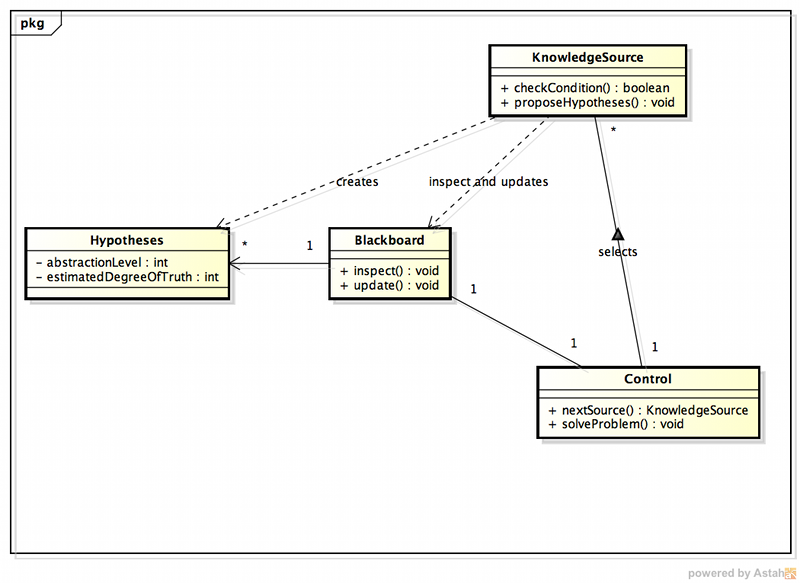
\includegraphics[width=\textwidth]{content/posa1/images/blackboard-class.png}
	\caption{ClassDiagram}
\end{figure}

::UML Diagramm von Seite 79 machen und etwas erklären::

\subsection*{Dynamics}


\begin{itemize}
	\item Main Loop der Control Component ist gestartet
	\item Die Control Componente ruft nextSource() auf um die nächste Knowledge Source auszuwählen
	\item nextSource() entscheidet mit Hilfe des Blackboards zuerst welche Knowledge Sources potentiell etwas beitragen können
	\item nextSource() ruft danach den condition-part jeder potentiellen Knowledge Source auf
	\item Die Control Componente entscheidet sich für eine Knowledge Source und eine Hypothese oder eine Menge von Hypothesen mit welchen gearbeitet wird
\end{itemize}

\begin{figure}[H]
	\centering
	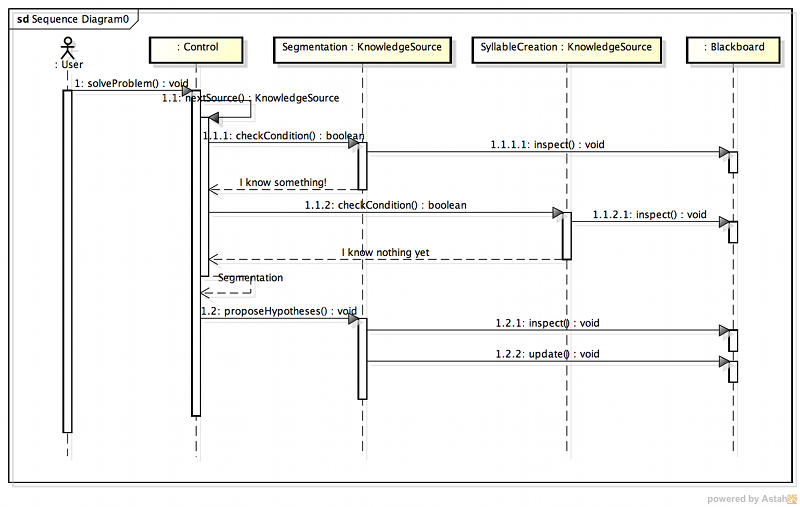
\includegraphics[width=\textwidth]{content/posa1/images/blackboard-sequence.png}
	\caption{SequenceDiagram}
\end{figure}

::UML Sequenz Diagramm von Seite 80 oder eigenes Beispiel::


\subsection*{Implementation}

:: Kann man noch endlos ausbauen... ::

\begin{enumerate}
	\item Definiere das Problem
	\item Definiere den Solution Space (Lösungsraum) für das Problem
	\item Zerlege den Lösungsprozess in Schritte
	\item Zerlege das Knowledge in speziallisierte Knowledge Sources
	\item Definiere ein Vocabulary für das Blackboard
	\item Spezifiere die Kontrolle des Systems
	\item Implementiere die Knowledge Sources
\end{enumerate}


\subsubsection*{Production System}


(OPS language???)

Bei dieser Variante werden Subroutinen als condition-action Regeln repräsentiert und die Daten liegen global im Speicher. Condition-action Regeln haben eine linke Seite, welche die Condition definiert und eine rechte Seite, welche die Action definiert. Die Action wird nur ausgeführt wenn die Condition erfüllt ist und die Regel selektiert wurde. Die Selektion wird von einem "conflict resolution module" vorgenommen.

\subsubsection*{Repository}


Diese Variante ist eine Verallgemeinerung des Blackboard Pattern. Die zentrale Datenstruktur wird Repository genannt. Das Repository Pattern definiert keine interne Control Component. Das Repository kann durch eine Benutzereingabe oder ein externes Programm kontrolliert werden. Eine traditionelle Datenbank kann als Repository betrachtet werden. Compiler können als Pipelines implementiert werden. Moderne Compiler benutzen allerdings ein Repository welches gemeinsame Informationen enthält, wie die Symboltabellen doer Abstract Syntax Trees (AST).

\subsection*{Known uses}


:: könnte man auch noch mehr ausbauen, falls einem Spracherkennungssystem aus den 70ern interessieren..? P. Sommerlad mag aber auch moderne Beispiele, Ideen? ::

\begin{itemize}
	\item HEARSAY-II: Ein Spracherkennungssystem aus den frühen 70ern. Es wurde als natürliches Sprachinterface für eine Literaturdatenbank entwickelt.
	\item HASP/SIAP: System um Gegnerische Uboote zu entdecken.
	\item Crysalis: Dreidimensionale Strukturen von Protein Molekülen mit Hilfe von Röntenstrahlung erkennen. -> Wikipedia Kristallstrukturanalyse http://de.wikipedia.org/wiki/Kristallstrukturanalyse
	\item Tricero: Ein System welches Flugzeugbewegungen überwacht. Das System erweitert die Blackboard Architektur um verteilte Berechnungen (distributed computing)
	\item Generalizations: zwischen 1977 und 1984 wurden Blackboardsysteme verallgemeinert um Frameworks zu bekommen, welche das erstellen von Blackboard-Anwendungen vereinfachen sollten.
	\item SUS: Software Understanding System. Das Ziel von SUS ist es, das Verständnis von Software zu unterstützen. Unter anderem mit der Suche nach wiederwendbaren Teilen.
\end{itemize}

\subsection*{Example Resolved}

:: Weglassen? Eigenes Beispiel? ::

\subsection*{Consequences}


Der Blackboard Ansatz geht auf die meisten Forces ein:

\begin{itemize}
	\item Experimentieren
	\item Austauschbarkeit und Wartbarkeit
	\item Wiederverwendbare Knowledge Sources
	\item Unterstützung für Fault Tolerance und Robustheit
\end{itemize}

\subsection*{Liablities}


\begin{itemize}
	\item Schwierig zu testen: kein deterministischer Algrothimus
	\item Keine Garantie für eine gute Lösung
	\item Schwierigkeit eine gute Control Strategie festzulegen
	\item Ineffizient: Viel overhead durch falsche Hypothesen
	\item Hoher Entwicklungsaufwand
	\item Keine Unterstützung für Parallelität: Potentielle parallelität von Knowledge Sources wird nicht verhindet, aber auch nicht gefördert. Die zentrale Datenstruktur des Blackboards muss synchronisiert werden
\end{itemize}

\begin{itemize}
	\item Schwierigkeit eine gute Control Strategie festzulegen
	\item Ineffizient: Viel overhead durch falsche Hypothesen
	\item Hoher Entwicklungsaufwand
	\item Keine Unterstützung für Parallelität: Potentielle parallelität von Knowledge Sources wird nicht verhindet, aber auch nicht gefördert. Die zentrale Datenstruktur des Blackboards muss synchronisiert werden
\end{itemize}

\begin{itemize}
	\item Hoher Entwicklungsaufwand
	\item Keine Unterstützung für Parallelität: Potentielle parallelität von Knowledge Sources wird nicht verhindet, aber auch nicht gefördert. Die zentrale Datenstruktur des Blackboards muss synchronisiert werden
\end{itemize}

